\documentclass{article}
\usepackage[utf8x]{inputenc}
\usepackage[margin=1in]{geometry}

\usepackage{graphicx}
\usepackage{enumitem}
\usepackage{hyperref}

\title{More Segment Trees}
\author{Kevin Geng}
\date{13 January 2017}

\usepackage{tikz}
\usetikzlibrary{calc,shapes.multipart,chains,arrows,positioning}
\tikzstyle{vertex}=[draw,fill=myseagreen,circle,minimum size=24pt,inner sep=0pt]
\definecolor{myseagreen}{RGB}{240,240,240}
\definecolor{mysalmon}{RGB}{240,180,170}

\begin{document}

\maketitle

\section{Lazy propagation}
With a segment tree, we can already handle the range sum query (RSQ) problems with a complexity of $O(\log n)$ for both queries and \textit{point updates}, or updates of individual elements. But what if we also wanted to perform \textit{range updates}, or updates of a range of elements? If we want to increment the value of $m$ contiguous elements, this will take $O(m \log n)$ time.

Fortunately, we can do better. With our current data structure, performing a range update will require modifying the values of $m$ elements, so we need to change our data structure. To avoid recursing all the way to the bottom of the tree for all $m$ elements, we can store some information in higher nodes instead.

Let's say we're performing a range update on the range $u$, and we're examining the segment $s$. The key insight is that if $s$ is contained within $u$, then we can simply set a \textit{lazy} value for $s$ instead of recursing on its children. When a lazy value is set, it means that the values of \textbf{each of} the children of that node should be incremented by that value.

\begin{figure}[h]
\center
{
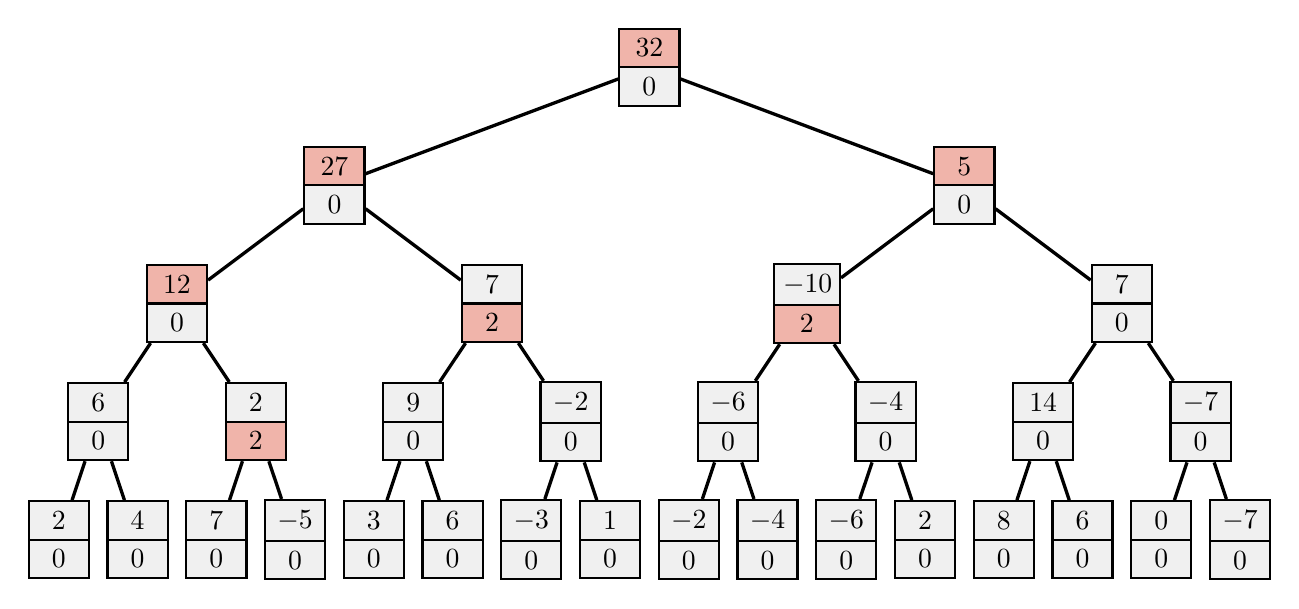
\begin{tikzpicture}[
  very thick,
  level 1/.style={sibling distance=80mm},
  level 2/.style={sibling distance=40mm},
  level 3/.style={sibling distance=20mm},
  level 4/.style={sibling distance=10mm},
  myrect/.style={
    draw,
    thick,
    rectangle split,
    rectangle split parts=2,
    rectangle split part fill={myseagreen, myseagreen},
    rectangle split part align=left,
    text width=3.5ex,
    text centered
    }
]
\node [myrect, rectangle split part fill={mysalmon, myseagreen}] (r){$32$\nodepart{two}0}
  child {
    node [myrect, rectangle split part fill={mysalmon, myseagreen}] (a) {27\nodepart{two}0}
    child {
      node [myrect, rectangle split part fill={mysalmon, myseagreen}] {12\nodepart{two}0}
      child {
        node [myrect] {6\nodepart{two}0}
        child {node [myrect] {2\nodepart{two}0}}
        child {node [myrect] {4\nodepart{two}0}}
      } 
      child {
        node [myrect, rectangle split part fill={myseagreen, mysalmon}] {2\nodepart{two}2}
        child {node [myrect] {7\nodepart{two}0}}
        child {node [myrect] {$-5$\nodepart{two}0}}
      }
    }
    child {
      node [myrect, rectangle split part fill={myseagreen, mysalmon}] {7\nodepart{two}2}
      child {node [myrect] {9\nodepart{two}0}
              child {node [myrect] {3\nodepart{two}0}}
        child {node [myrect] {6\nodepart{two}0}}
      }
      child {node [myrect] {$-2$\nodepart{two}0}
              child {node [myrect] {$-3$\nodepart{two}0}}
        child {node [myrect] {1\nodepart{two}0}}
      }
    }
  }
  child {
    node [myrect, rectangle split part fill={mysalmon, myseagreen}] {$5$\nodepart{two}0}
    child {
      node [myrect, text width=4ex, rectangle split part fill={myseagreen, mysalmon}] {$-10$\nodepart{two}2}
      child {node [myrect] {$-6$\nodepart{two}0}
              child {node [myrect] {$-2$\nodepart{two}0}}
        child {node [myrect] {$-4$\nodepart{two}0}}}
      child {node [myrect] {$-4$\nodepart{two}0}
              child {node [myrect] {$-6$\nodepart{two}0}}
        child {node [myrect] {$2$\nodepart{two}0}}}
    }
    child {
      node [myrect] {7\nodepart{two}0}
      child {node [myrect] {14\nodepart{two}0}
              child {node [myrect] {8\nodepart{two}0}}
        child {node [myrect] {6\nodepart{two}0}}}
      child {node [myrect] {$-7$\nodepart{two}0}
              child {node [myrect] {0\nodepart{two}0}}
        child {node [myrect] {$-7$\nodepart{two}0}}}
    }
  };

\end{tikzpicture}
}
\caption{Example of a segment tree with lazy values stored underneath. The highlighted values reflect the values updated after calling $update(3, 12, 2)$. \textit{Credit: Samuel Hsiang.}}
\end{figure}

However, if we encounter a lazy value while performing a query or an update, however, we need to push the value by moving the lazy value into its children, and updating the current node's sum correspondingly. But because we only push once per node, these operations still only take $O(\log n)$.

We can also use this technique to implement the range minimum query (RMQ) problem. A full implementation of both is provided by the solution to Counting Haybales (USACO December 2015, Platinum) at \url{http://www.usaco.org/current/data/sol_haybales_platinum_dec15.html}.


\section{Two-dimensional segment trees}

\subsection{Problem statement}

\begin{itemize}[leftmargin=0pt]
\item[\label={}]
%{\setlength{\parindent}{0cm}
%\setlength{\parskip}{\baselineskip}
\textit{Mowing the Field} (USACO January 2016, Platinum)

Farmer John is quite reliable in all aspects of managing his farm, except one: he is terrible at mowing the grass in a timely fashion. He only manages to move the mowing machine once per day, in fact. On day 1, he starts at position $(x_1,y_1)$ and on day $d$ he mows along a straight segment to the position $(x_d,y_d)$, moving either horizontally or vertically on the 2D map of his farm; that is, either $x_d = x_{d−1}$, or $y_d = y_{d−1}$. FJ alternates between horizontal and vertical moves on successive days.

So slow is FJ's progress that some of the grass he mows might grow back before he is finished with all his mowing. Any section of grass that is cut in day $d$ will reappear on day $d+T$, so if FJ's mowing path crosses a path he cut at least $T$ days earlier, he will end up cutting grass at the same point again. In an effort to try and reform his poor mowing strategy, FJ would like to count the number of times this happens.

Please count the number of times FJ's mowing path crosses over an earlier segment on which grass has already grown back. You should only count "perpendicular" crossings, defined as a point in common between a horizontal and a vertical segment that is an endpoint of neither.

(Bounds: $T \leq N \leq 100,000$ and $x_i, y_i < 1,000,000,000$)

\end{itemize}
%}

\subsection{Initial solution}
Let's start by examining a similar problem: what if the grass did not grow back (or if $T = N$)? Then this problem would be equivalent to finding intersecting lines, a standard line-sweep problem. We might solve this by using a binary search tree as an \textit{active set} denoting the horizontal lines present at the current $x$ position, which we update as we move the sweep line from left to right. (\textit{Nota bene:} We are sweeping through $x$ values, not through time.)

However, this approach does not provide an obvious way to count only the elements within time $T$ of a specified time $t$. We could attempt to solve this by iterating through the elements in the active set, and checking their times individually. However, given the bounds of the problem, this $O(N^2 \log N)$ algorithm is too slow even with an extended time limit of 5 seconds.

\subsection{Adding a segment tree}
Let's consider the problem from another angle. What if we built one binary search tree for each value of $T$? Obviously, this is extremely slow. For each query, we would need to process $2T-1$ of these trees, for each of the time values that might be affected.

However, each of these query operations will be on a continuous range of $2T-1$ time values. This motivates us to use a segment tree in the \textit{time dimension}, on which we can perform range queries! (We can also use a Fenwick tree to save memory.) Instead of storing an integer value, each of the nodes stores a binary search tree. Now, we can query our range of $2T-1$ times in $O(\log N)$. This reduces the total complexity to $O(N \log^2 N)$, which is fast enough to pass.

The solution provided by USACO uses a segment tree (which they call a \textit{range tree}) for the second dimension instead of a binary search tree. That's because the goal is to count the number of elements between two points, which can also be implemented using range sum query. However, because the max coordinate is one billion, the segment tree is dynamically allocated to save memory --- using an actual tree structure rather than an array-based one. The code takes some time to understand, but you can find it at \url{http://www.usaco.org/current/data/sol_mowing_platinum_jan16.html}.

\end{document}
